\Chapter{INTRODUCTION}
\label{intro}

An equation:
\al{eq:lm}{\Ex(\y)=\X\bb}

A reference \citep{Tibshirani1996}.

A figure.
\begin{figure}[ht!]
 \centering
 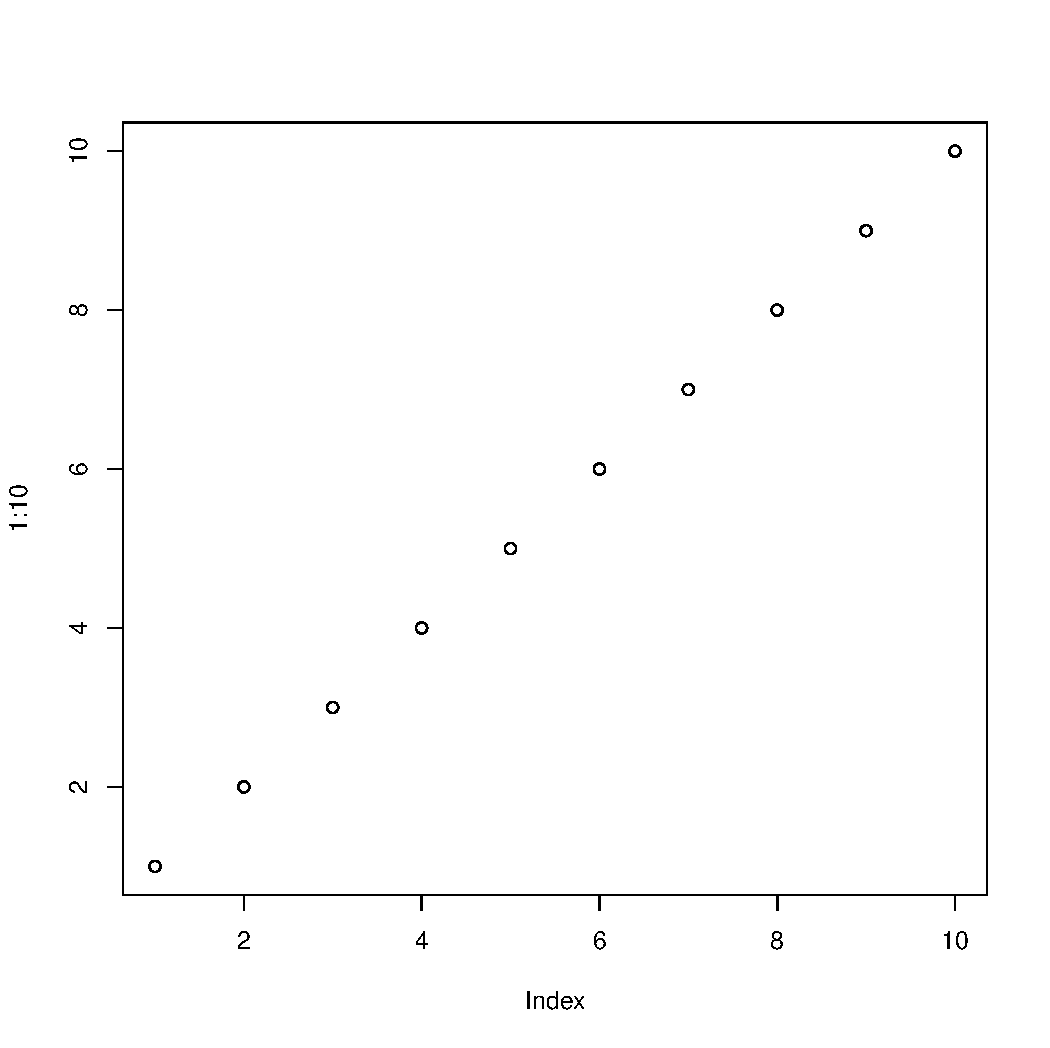
\includegraphics[width=0.6\textwidth]{fig1}
 \caption[Short caption]{\label{fig:fig1}Short caption.  More caption.}
\end{figure}

A table.
\begin{table}[ht!]
 \ttabbox
 {\caption{\label{tab:tab1}Tables can only have short captions.}}
 {\begin{tabular}{cccc}
\hline
 & A & B & C \\
\hline
A & 1 & 2 & 3 \\
B & 4 & 5 & 6 \\
C & 7 & 8 & 9 \\
\hline
\end{tabular}}
\end{table}
